\pref{def:PH} introduces the Process Hitting~(PH)~\cite{PMR10-TCSB}
which allows to model a finite number of local levels,
called \emph{processes},
grouped into a finite set of components, called \emph{sorts}.
A process is noted $a_i$, where $a$ is the sort's name,
and $i$ is the process identifier within sort $a$.
At any time, exactly one process of each sort is \emph{active},
and the set of active processes is called a \emph{state}.

The concurrent interactions between processes are defined by a set of \emph{actions}.
Each action is responsible for the replacement of one process by another of the same sort
conditioned by the presence of a set of other process, at least one, in the current state.
An action is denoted by $\PHfrappe{A}{b_j}{b_k}$, which is read as "all the processes in $A$ cooperate to \emph{hit} $b_j$ and make it \emph{bounce} to $b_k$'',
where $b_j$, $b_k$ are processes of sorts $b$.
and we call the processes of $A$, $b_j$ and $b_k$  respectively \emph{hitters}, \emph{target} and
\emph{bounce} of the action.
We also call a \emph{self-hit} any action with one hitter such that the hitter and target sorts are the same,
that is, of the form: $\PHfrappe{b_j}{b_j}{b_k}$.

The PH is therefore a restriction of asynchronous automata networks, where each transition
changes the local state of exactly one automaton,
and is triggered by the local states of at most two distinct automata.
This restriction on the actions was chosen to permit
the development of efficient static analysis methods
based on abstract interpretation~\cite{PMR12-MSCS}.

\begin{definition}[Process Hitting]\label{def:PH}
  A \emph{Process Hitting} is a triple $(\PHs,\PHl,\PHa)$ where:
  \begin{itemize}
    \item  $\PHs = \{a,b,\dots\}$ is the finite set of \emph{sorts};
    \item  $\PHl = \prod_{a\in\PHs} \PHl_a$ is the set of \emph{states} where
      $\PHl_a = \{a_0,\dots,a_{l_a}\}$
      is the finite set of \emph{processes} of sort $a\in\Sigma$
      and $l_a$ is a positive integer, with $a\neq b\Rightarrow \PHl_a \cap \PHl_b = \emptyset$;
    \item $\PHa$ = \{ $\PHfrappe{A}{b_j}{b_k}$ with $A \in \PHl^{\diamond} \wedge b \in \PHs \wedge b_j \neq b_k \wedge$ if $b_j \in A \Rightarrow A=b_j$\} is the finite set of \emph{actions}.
    With $\PHl^{\diamond}$ the set of all the sub-states of $\PHl$.    
      %$\PHa$ = \{ $\PHfrappe{A}{b_j}{b_k}$ with $A \in \PHl^{\diamond} \wedge b \in \PHs \wedge b_j \neq b_k \wedge$ if $b_j \in A \Rightarrow A=b_j$ \}.With $\PHl^{\diamond}$ the set of all the sub-states of $\PHl$. 
  \end{itemize}
\end{definition}

\begin{example}
\pref{fig:ph} represents a PH model with five sorts: $a$, $b$, $c$, $d$ and $e$.
\begin{figure}[!h]
  \centering
  \scalebox{1.3}{
  \begin{tikzpicture}[apdotsimple/.style={apdot}]

   \TSort{(3.5,0.5)}{a}{2}{r}
    \TSort{(3,4.5)}{b}{3}{t}
    \TSort{(7,1)}{e}{2}{r}  
    \TSort{(0,3)}{c}{2}{r}
    \TSort{(0.5,0)}{d}{2}{r}
    
    \THit{d_1}{selfhit}{d_1}{.north west}{d_0}
       
   % \THit{e_1}{selfhit}{e_1}{.north east}{e_2}
% b en 3 niveaux avec un selfhit de 1 à 2
   \THit{d_0}{}{a_0}{.west}{a_1}
   \TActionPlur{a_1, b_1}{e_0.north west}{e_1.west}{}{5.5,2.5}{left}
   \TActionPlur{a_1, c_1}{b_0.south}{b_1.south west}{}{2,3}{right}

    \path[bounce, bend right]
      % \TBounce{d_1}{}{d_0}{.north}
   \TBounce{d_1}{}{d_0}{.north west}
  %    \TBounce{e_1}{}{e_2}{.north east}
    ;
   \path[bounce, bend left]
   \TBounce{a_0}{}{a_1}{.south west}
%	\TBounce{z_0}{bend left=90}{z_1}{.south east}
    ;
    \TState{a_0, b_0, c_1, d_0, e_0}
  \end{tikzpicture}
  }
  \caption{\label{fig:ph}
An example of PH model with five sorts: $a$, $b$, $c$, $d$ and $e$. Boxes represent the sorts, the biological components, circles represent the processes (component levels), and the actions that model the dynamic behavior are depicted by pairs of arrows in solid and dotted lines. $a$, $d$, $c$ and $e$ are all either at level $0$ or $1$, and the sort $b$ has $3$ levels $0$, $1$, $2$. The grayed processes stand for the possible initial state $\PHstate{a_0, b_0, c_1, d_0, e_0}$.
  }
\end{figure}

\end{example}

A state of the network is a set of active processes containing a single process of each sort.
The active process of a given sort $a \in \PHs$ in a state $\PHst \in \PHl$
is noted $\PHget{\PHst}{a}$.
For any given process $a_i$ we also note: $a_i \in \PHst$ if and only if $\PHget{\PHst}{a} = a_i$. It means that the biological component $a$ is in the condition labeled $i$ within state $\PHst$.

\subsection{Attractors in Process Hitting}

The study of the dynamics of biological networks was the focus of many works, explaining the diversity of network modelings and the different methods developed in order to identify attractors \cite{skodawessely2011finding, zhang2007algorithms, mushthofa2014asp, akutsu2012finding, berntenis2013detection}.
In this paper we focus on a main property in automata networks: the steady states, the cycles and the attractors . %Then we verify the reachability of these attractors. \\
In the following, we consider an automata networ modeled in PH $\PH=(\PHs,\PHl,\PHa)$,
and we formally define these properties.
%How to verify them with the help of ASP is the subject of the rest of this paper.
%and explain how they could be verified on a such network.

\begin{definition} [Playable action]
\label{def:playableAction}
Let $\PH = (\PHs,\PHl,\PHa)$ be a Process Hitting and $\PHst \in \PHl$ a state of $\PH$.
We say that the action $h = \PHfrappe{a_i}{b_j}{b_k} \in \PHa$
is \emph{playable in state $\PHst$} if and only if
$A \subseteq \PHst$ and $b_j \in \PHst$ (\ie$ \forall a_i \in A$, $\PHget{\PHst}{a} = a_i$ and $\PHget{\PHst}{b}=b_j$).
\end{definition}

\Emna{A relire} We can consider that the playable actions in a PH state are equivalent to the transitions from a state in the state transition graph.

 At each state, a couple of actions are playable and they are resposible of the evolution of the system from one state to another.

\begin{Lemma}
The resulting state after playing an action $h= \PHfrappe{A}{b_j}{b_k}$ in a state $\PHst$
is called a \emph{successor} of $\PHst$ and
is denoted by $(\PHst \play h)$,
where $\PHget{(\PHst \play h)}{b} = b_k$ and
$\forall c \in \PHs, c \neq b \Rightarrow \PHget{(\PHst \play h)}{c}=\PHget{\PHst}{c}$.
\end{Lemma}

Since we are considering only \emph{asynchronous} updating (\Emna{ref asynchrone}), only one component could change its expression level from a state to its successor (i.e play only one action at each step). In the following, if $\PHst \in \PHl$ is a state,
we call \emph{scenario from~$\PHst$}
any sequence of successively states from $\PHst$ denoted by $\Sce(\PHst)$. \\

In the example of PH model of \pref{fig:ph}, if we consider an initial state $\PHst_0 = \PHstate{a_0, b_0, c_1, d_1, e_0}$ or knowing the sorts order, $\PHst_0 = (0, 0, 1, 1, 0)$ the sequence of the successively states of $\PHst_0$ denoted by $\Sce(\PHst_0)$ is expressed above: \\
(0, 0, 1, 1,0) $\rightarrowtail$ (0, 0, 1, \underline{0}, 0) $\rightarrowtail $ (\underline{1}, 0, 1, 0, 0) $\rightarrowtail$ (1, \underline{1}, 1, 0, 0) $\rightarrowtail$ (1, 1, 1, 0, \underline{1}). 

A \emph{fixed point}, also called \emph{steady state},
is a state which has no successor,
as given in \pref{def:fixpoint}.
Such states have a particular interest as they denote states in which the model
stays indefinitely,
and the existence of several of these states denotes a switch in the dynamics~\cite{wuensche1998genomic}.

\begin{definition}[Fixed point]
\label{def:fixpoint}
  A state $\PHst \in \PHl$ is called a \emph{fixed point}
  (or equivalently \emph{steady state})
  if and only if it has no successors.
  In other words, $\PHst$ is a fixed point if and only if no action is playable in this state:
$$ \forall \PHfrappe{A}{b_j}{b_k} \in \PHa, A \notin \PHst \vee b_j \notin s \enspace. $$
\end{definition}

A finer and more general dynamical property consists in
the notion of \emph{attractors}.
Such a property, formally expressed in \pref{def:attractor},
states that a set of states that are connected and in which the system loops indifinetly (See \ref{fig:transition-graph}). \\

%states that starting from a given initial state, it is possible
%to reach a given goal, that is, a state that contains a process
%or a set of processes.
%Checking such a dynamical property is considered difficult
%as, in usual model-checking techniques,
%it is required to build (a part of) the state graph,
%which has an exponential complexity.

\begin{definition}[Cycle or Loop]
\label{def:cycle}
A set of states $\mathbf{C} = \bigcup\limits_{i=1}^{N} \PHst_{i}$ is called a \emph{cycle} of size $N$ if and only if $\forall \PHst \in \mathbb{C}, \PHst \in \Sce(\PHst) $.
\end{definition}

\Emna{du contenue à propos les cycles}
Some \emph{scenarios} of a network eventually converges to either a single state, or a cycle of states, called \emph{attractor}. 

\begin{definition}[Attractor]
\label{def:attractor}
A set of $N$ states $\Delta = \bigcup\limits_{i=1}^{N} \PHst_{i}$ is called an \emph{attractor} of size $N$ if and only if $\Delta$ is a cycle and $\forall h \in \PHa $ playable in $\PHst \in \Delta$, $(\PHst \play h) \in \Delta$.
\end{definition}

If the system evoluate and attend an a state of an attractor, so it wil cycle infinitely into the attractor states.
We can confuse an attractor of 1-size with a fixed point (i.e steady state). \\

The aim of this paper is to focus on the resolution of issues related to the previous definitions:
we give algorithms enumerating all fixed points (\pref{sec:fixpoint})
and all attractors (\pref{sec:attractors}). We propose later to tackle the simulation of a PH model in ordor to verify which ones of these attractors are reachable.

\begin{figure}[h]
   \caption{\label{fig:transition-graph} A state transition graph of a PH model with 3 sorts (one sort with two levels $0$ or $1$ and two other sorts have three levels $0$, $1$ and $2$). This graph contains two attractors (size 2 and size 4) and one fixed point}
   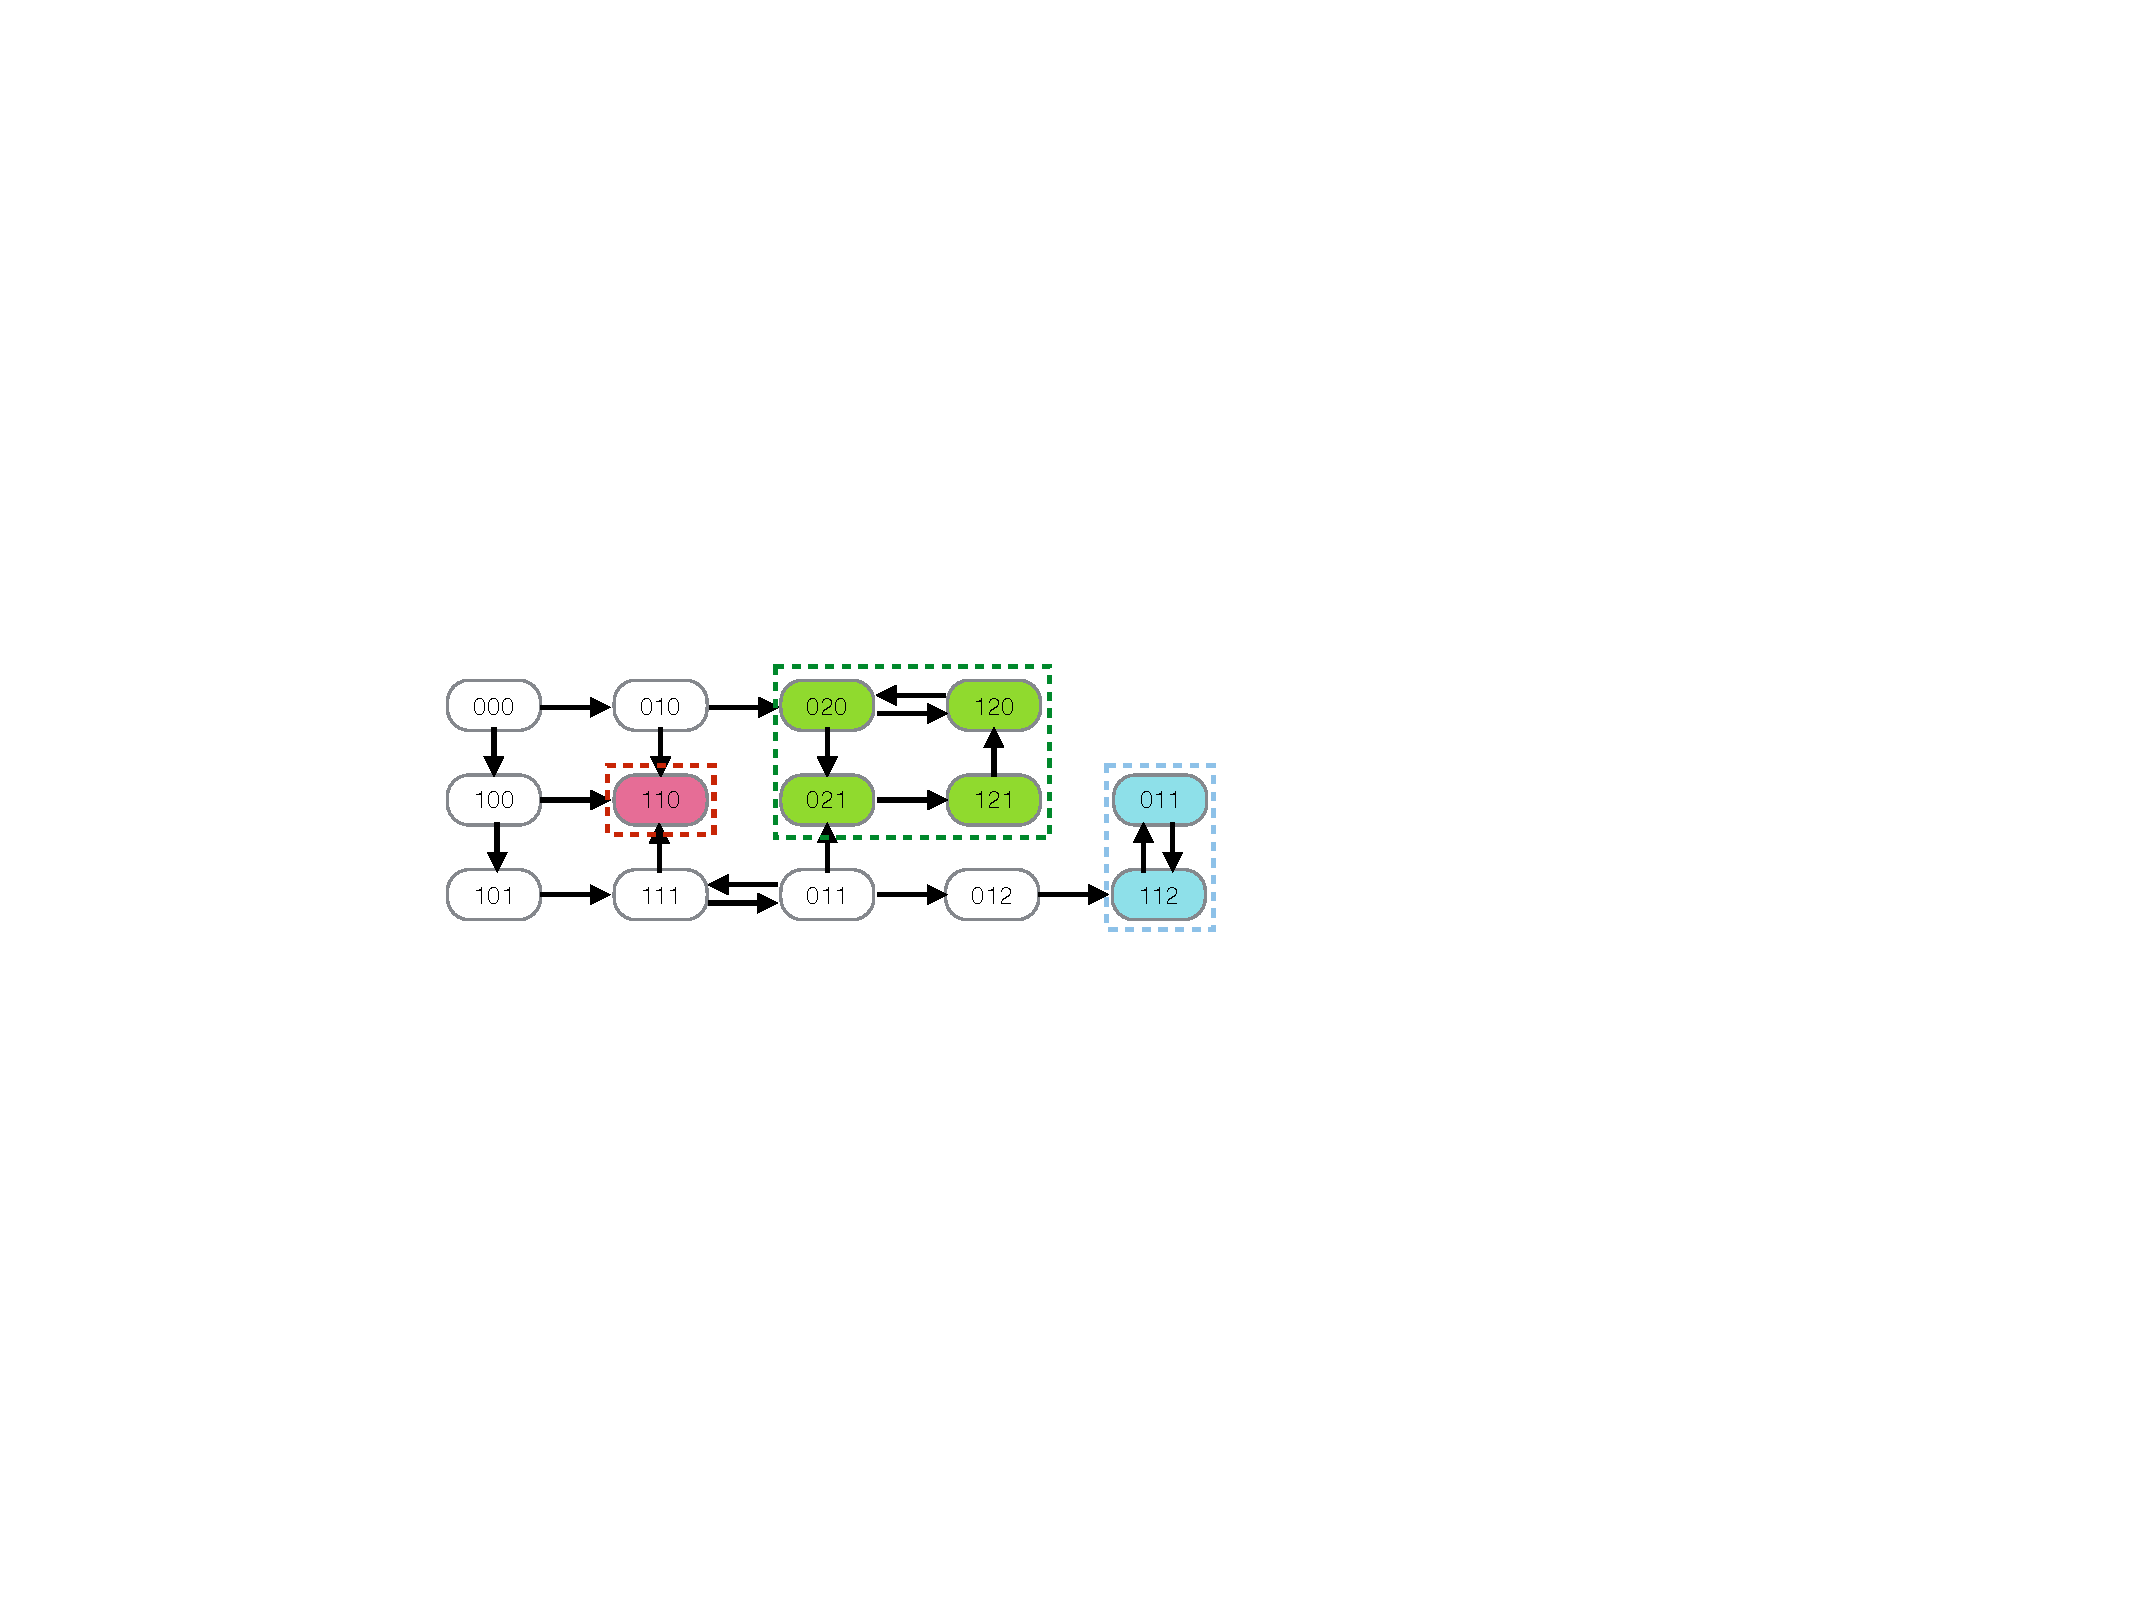
\includegraphics{figures/transition-graph.pdf}
\end{figure}
